\documentclass[UTF8]{ctexart}
\usepackage{bookmark}
\usepackage{geometry}
\usepackage{hyperref}
\geometry{a4paper,scale=0.8}
\usepackage{ctex}
\usepackage{booktabs}
\usepackage{array}
\usepackage{fancyhdr}
\usepackage{physics}
\pagestyle{fancy}
\fancyhf{}
\renewcommand\footrulewidth{1pt}
\lhead{\textit{王铠泽}}
\rhead{\textit{PB18020766}}
\chead{\href{mailto:volar@mail.ustc.edu.cn}{\textit{volar@mail.ustc.edu.cn}}}
\rfoot{\href{http://en.ustc.edu.cn/}{\textit{中国科学技术大学}}}
\lfoot{\textit{\today}}
\usepackage{graphicx}
\usepackage{float}
\usepackage{subfigure}
\fancyfoot[C]{\textit{\thepage}}


\begin{document}

	\centering\textbf{\LARGE{计算物理A第十九次作业}}
	
	
	\textit{王铠泽}\qquad\textit{ PB18020766}
	
		
	\section{作业题目}
	
	11111111
	
	\section{实现方法和原理}
	
	22222222
	
	\section{程式说明}
	
	22222222
	
	\section{计算结果}
	
	\begin{table}[H]
			\centering
			\begin{tabular}{@{}lllll@{}}
				\toprule
				12412& 421342 &41232  & 412231 &  \\ \midrule
				111&  333&  4324&  312&  \\
				1323&  132&  132&  123&  \\
				123&  1323&  1231&  312&  \\ \bottomrule
			\end{tabular}
		\end{table}

%	\begin{figure}[H]
%	\centering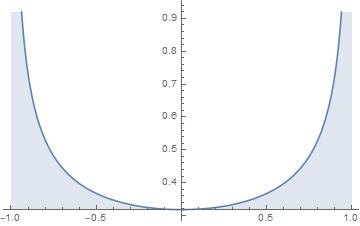
\includegraphics[width=2in]{1.jpg}
%	\caption{something}\label{fig:1}
%	\end{figure}
%		
%	\begin{figure}[H]
%		\centering  %图片全局居中
%		\subfigure[name1]{
%			\label{Fig.sub.1}
%			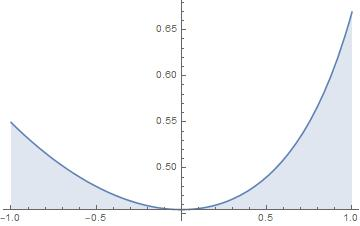
\includegraphics[width=0.45\textwidth]{2.jpg}}
%		\subfigure[name2]{
%			\label{Fig.sub.2}
%			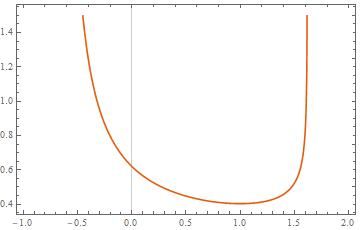
\includegraphics[width=0.45\textwidth]{3.jpg}}
%		\caption{Main name}
%		\label{Fig.main}
%	\end{figure}

	\section{总结}

	524757673

\end{document}